\chapter{Velocity Estimates in Vegetated Lateral Cavities}
\label{chap:art3}
In this chapter, the second topic of the dissertation is further developed in a published conference paper. The objective of this paper was to develop a simple numerical method capable of estimating the flow and the mass exchange between a lateral cavity and the main channel. Differently of the previous chapter, this paper introduces an open source approach to the problem, making the model further accessible to the general public. Also, the numerical model was further developed to account the mass transfer between the regions.

The original paper was published in the 'XIII Encontro Nacional de Águas Urbanas', on October 2020, Porto Alegre, Brazil.
\section*{Authors}
\begin{itemize}
    \item Luiz Eduardo Domingos de Oliveira \footnote{Federal University of Mato Grosso do Sul}
    \item Taís Natsumi Yamasaki \footnotemark[1]
    \item Johannes Gérson Janzen \footnotemark[1]
    \item Carlo Gualtieri \footnote{University of Naples Federico II}
\end{itemize}
\addcontentsline{toc}{section}{Abstract}
\section*{Abstract}
Lateral cavities are a type of transient storage zones that occur in riverine systems. They play an important role in mass transport processes, especially due to a higher residence time. In this study, a numerical simulation of flow past a lateral cavity with vegetation was performed to assess the impact of the vegetation on the cavity hydrodynamics. The vegetation drag was introduced in a simplified method, as it was modelled as an anisotropic porous medium. The model could reproduce the experimental results at a reduced computational cost and can be considered a study platform for future studies.

\noindent\textbf{Keywords:} Lateral Cavities; Vegetation; Computational Fluid Dynamics (CFD).

\section{Introduction}
In rivers, lateral cavities are regions laterally attached to the channel, where the dynamics of the flow are characterised by slow velocities, increased mass residence time and the presence of re-circulations \cite{chang_constantinescu_park_2006}. The exchange processes between the unaltered channel (main channel) and the cavity occur solely by an interface in which the mass and momentum relationships occur. Since there is an increased residence time within the cavity volume due to the lower velocity magnitudes, this region favours sedimentation processes and vegetation growth. The presence of vegetation in the cavity alters the hydrodynamics and the interface exchanges \cite{xiang2019}.

The importance of lateral cavities in ecosystems is significative. For instance, the reduced velocities and the recirculation promote higher rates of sediments deposition and organic matter \cite{Juez2018} and also creates a favourable lentic environment to fish populations \cite{Landwust2006}. Furthermore, lateral cavities promote the temporary storage of nutrients and contaminants, eg. heavy metals \cite{Argerich2011,xiang2019}, what make this structure a viable place for absorption and treatment of these substances.

Since the vegetation occurs naturally in lateral cavities and that its presence alters the dynamics of the flow. In this study, we aimed to simulate numerically the flow in a single rectangular lateral cavity with the presence of emergent vegetation, to comprehend the effects of vegetation inside the lateral cavity.

\section{Methods}
The modelled geometry consists in a channel reach with a lateral cavity \ref{fig:art3:compDomain}. The main channel had a length of $L_{ch}=1.25$m (x-axis), a width of $W_{ch}=0.30$m (y-axis) and depth of $H_{ch}=0.10$m (z-axis). The lateral cavity had a lengh of $L_{cv}=0.25$m, width of $W_{cv}=0.15$m and depth of $H_{cv}=0.10$m. These dimensions were based on the laboratory experiments of \textcite{xiang2019}. The mean velocity at the main channel was $U=0.101$m/s, which corresponds to a Reynolds number of 9000 (turbulent flow).

\begin{figure}[!ht]
\centering
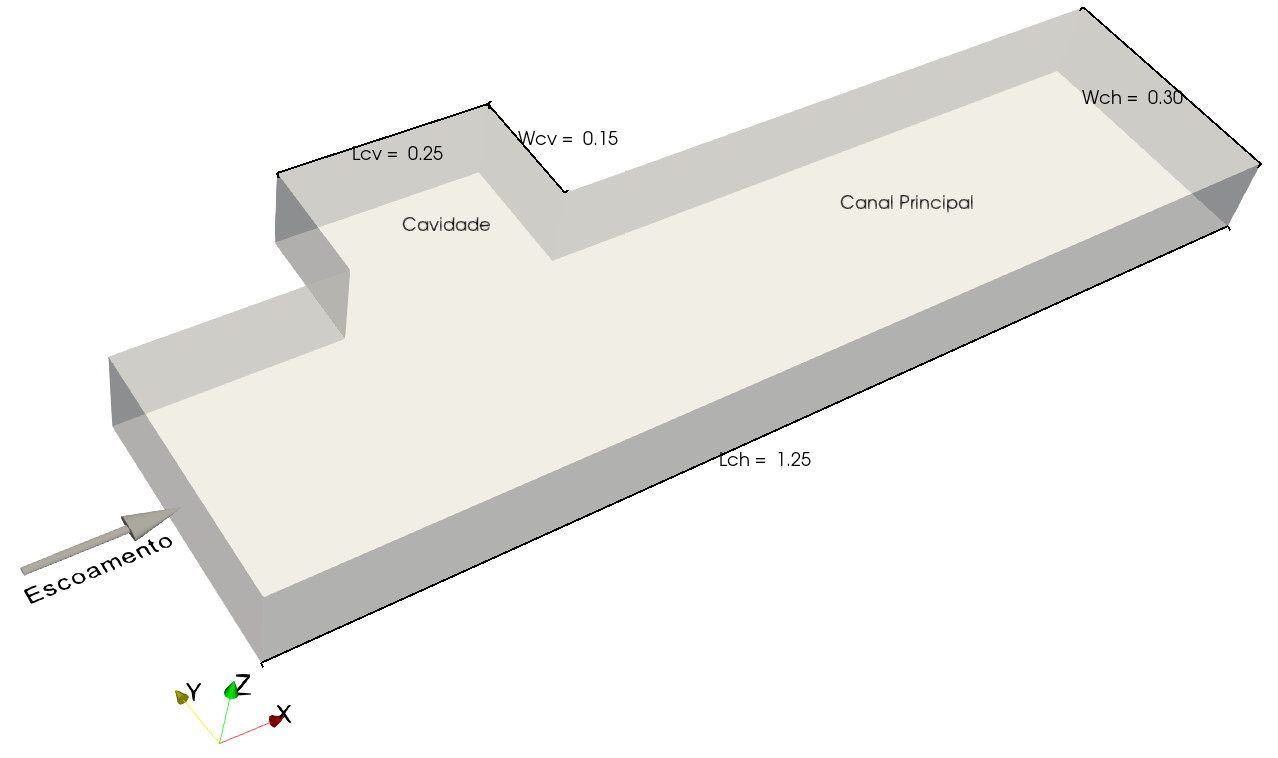
\includegraphics[width=\linewidth]{../images/art3/imgEst1.png}
\caption{Numerical domain. The coordinate origins ($x,y,z=0$) is at the lower left corner of the picture. The inlet surface is at $x=0$m, outlet at $x=0.75$m and the cavity is between $0.25<x (m)<0.50$, connected to the channel.}
\label{fig:art3:compDomain}
\end{figure}

The computational domain was calculated with the finite volume method and thus requires the discretisation of the geometry into a mesh. The geometry was divided into four blocks: cavity, upstream channel, downstream channel and middle channel. The mesh was made exclusively of orthogonal hexahedrons. The block within the cavity was divided into 80 divisions in both x and y directions, the elements close to the wall were refined to increase the accuracy of the model, the total growth rate was kept at a constant of 2. The entire domain was divided 40 times in the z-axis with a total growth rate, from the bottom, of 41. The mesh totalised in 1,408,000 elements.

At the free surface ($z=0.10$m) and at the cut surface ($y=0$m) the slip wall boundary condition was applied. The inlet surface ($x=0$m) was modelled through a pre-developed profile of velocities and reynolds stresses that were previously calculated in a periodic flow separated from this main simulation. This data was mapped to feed the synthetic vortex boundary condition applied (\textit{turbulentDFSEMInlet}). The outlet ($x=1.25$m) was treated as a zero gradient and all the other surfaces of the domain were treated as no-slip smooth walls. The wall function \textit{nutUSpalldingWallFunction} was implemented in all walls to compute the variation of turbulence viscosity in the domain. Lastly, the model large eddy simulation (LES) was implemented, with a sub-grid filter wall-adapting  local eddy-viscosity (WALE) to account the effects of turbulence in the channel.

The emergent vegetation inside the cavity was based in the second case of \cite{xiang2019} study. The model used to describe the resistance caused by the vegetation was through a porous media calculated using the Darcy-Forchheimer equation, in which the inertial ($f$) and viscous ($d$) drag coefficients were calculated using the Ergun formulation in the x and y directions. The anisotropy caused by vegetation was considered in the z direction, where the drag coefficients were calculated using the method of \cite{oldham2001}.

The open-source package OpenFOAM (version 1912) was used to calculate the computational model. The chosen calculation module of the pressure-velocity coupling was the PIMPLE, which uses both the transient formulation of the PISO with the permanent of SIMPLE. The numerical schemes chosen were of second-order to provide the necessary precision of LES. The time-steps were defined in an variable way assuring that the maximum Courant number was $0.90$.

\section{Results and Discussion}
The mean velocities (time averaged) calculated from the model, had lower magnitudes than the main channel (\ref{fig:art3:velCont}). A single circulation system was observed in the lateral cavity (\ref{fig:art3:streamlines}), as it was expected for aspect ratios between $0.5<W/L<1.5$ \cite{Uijttewaal2001}. The origin of this circulation occurs in the momentum transfer from the main channel to the lateral cavity, as the flow occurs to the right, the circulation was in an anti-clockwise direction. At the upper left corner of the cavity an even higher reduction was observed, this occurs because of the path that the jet passes that starts at the inferior right region and follows it way deducting energy to the vegetation drag.

In energy exchange terms, the model was able to capture the interface between a cavity and the main channel (\ref{fig:art3:velCont}), this could be visualised through the steady velocity gradient that forms from the lower left corner of the cavity. From this point, the vortexes are dissipated and may enter the cavity or be ejected out to the main channel (\ref{fig:art3:vectors}), similar to the process of multiple cavities inside the main channel (groynes) \cite{uijttewaal2005}. Still in this figure, we could observe the difference in magnitude of the vectors, what reinforces the idea that the vegetated lateral cavities favour mass deposition due to its low velocities.

\begin{figure}[!ht]
\centering
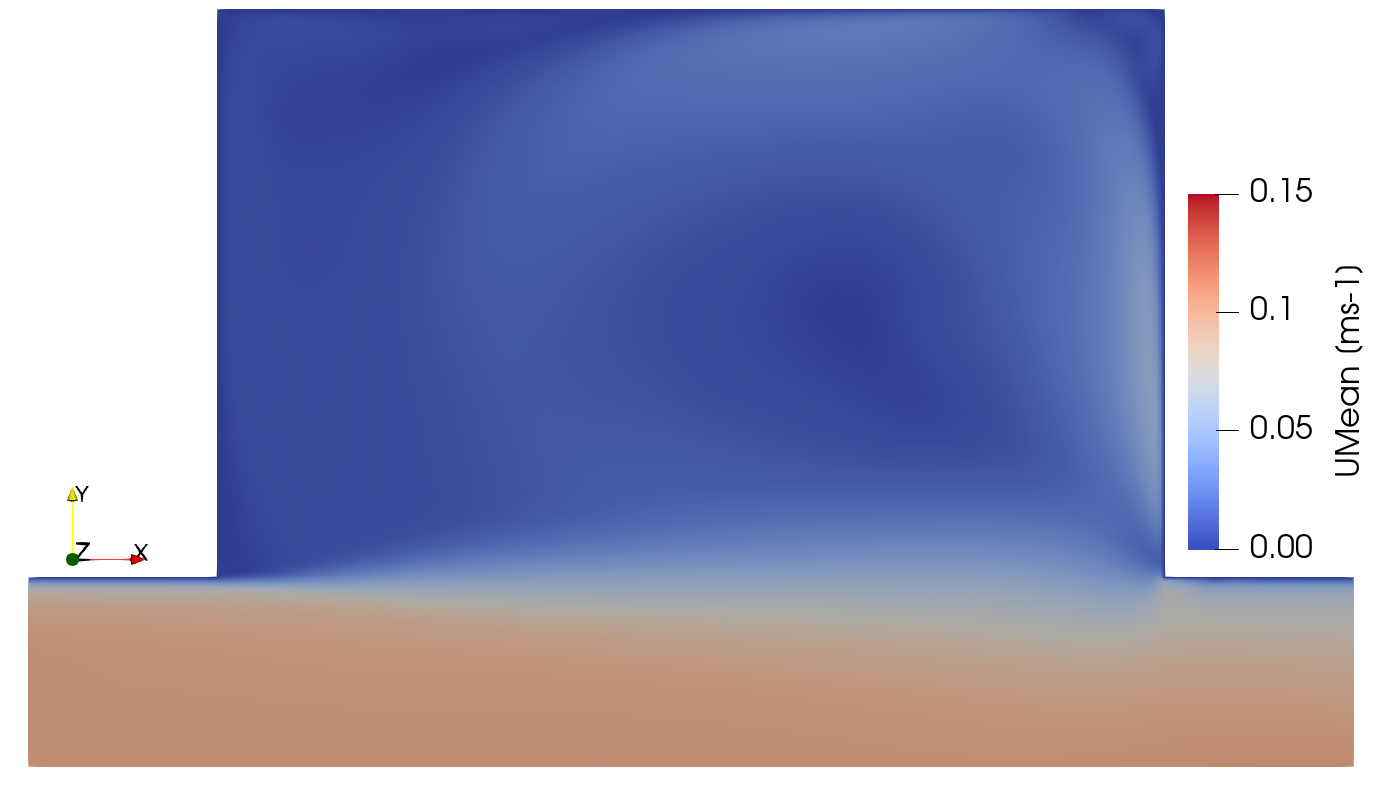
\includegraphics[width=\linewidth]{../images/art3/imgEst2.png}
\caption{Mean velocity contour in the XY plane, in $z=0.6H$}
\label{fig:art3:velCont}
\end{figure}
\begin{figure}[!ht]
\centering
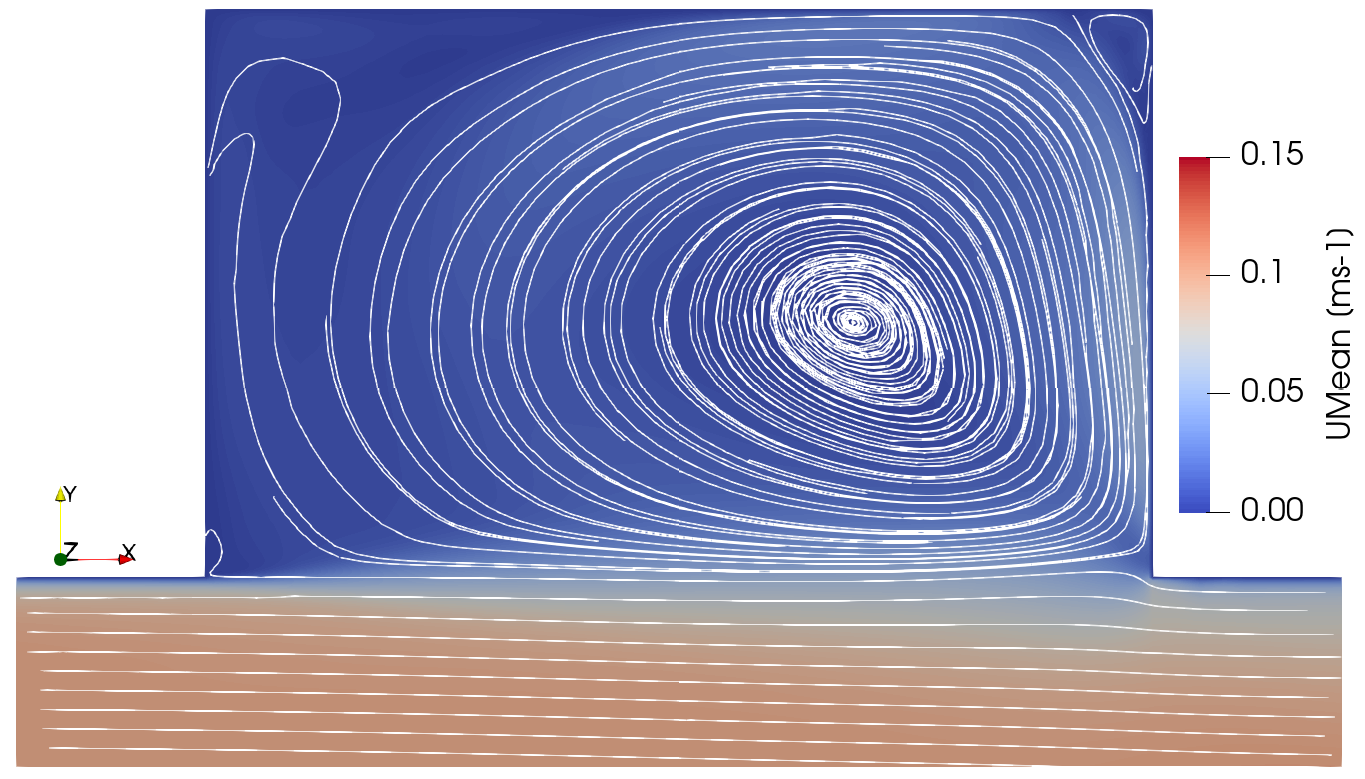
\includegraphics[width=\linewidth]{../images/art3/imgEst3.png}
\caption{Mean velocity contour in the XY plane, in $z=0.6H$ with additional streamlines associated to the flow.}
\label{fig:art3:streamlines}
\end{figure}
\begin{figure}[!ht]
\centering
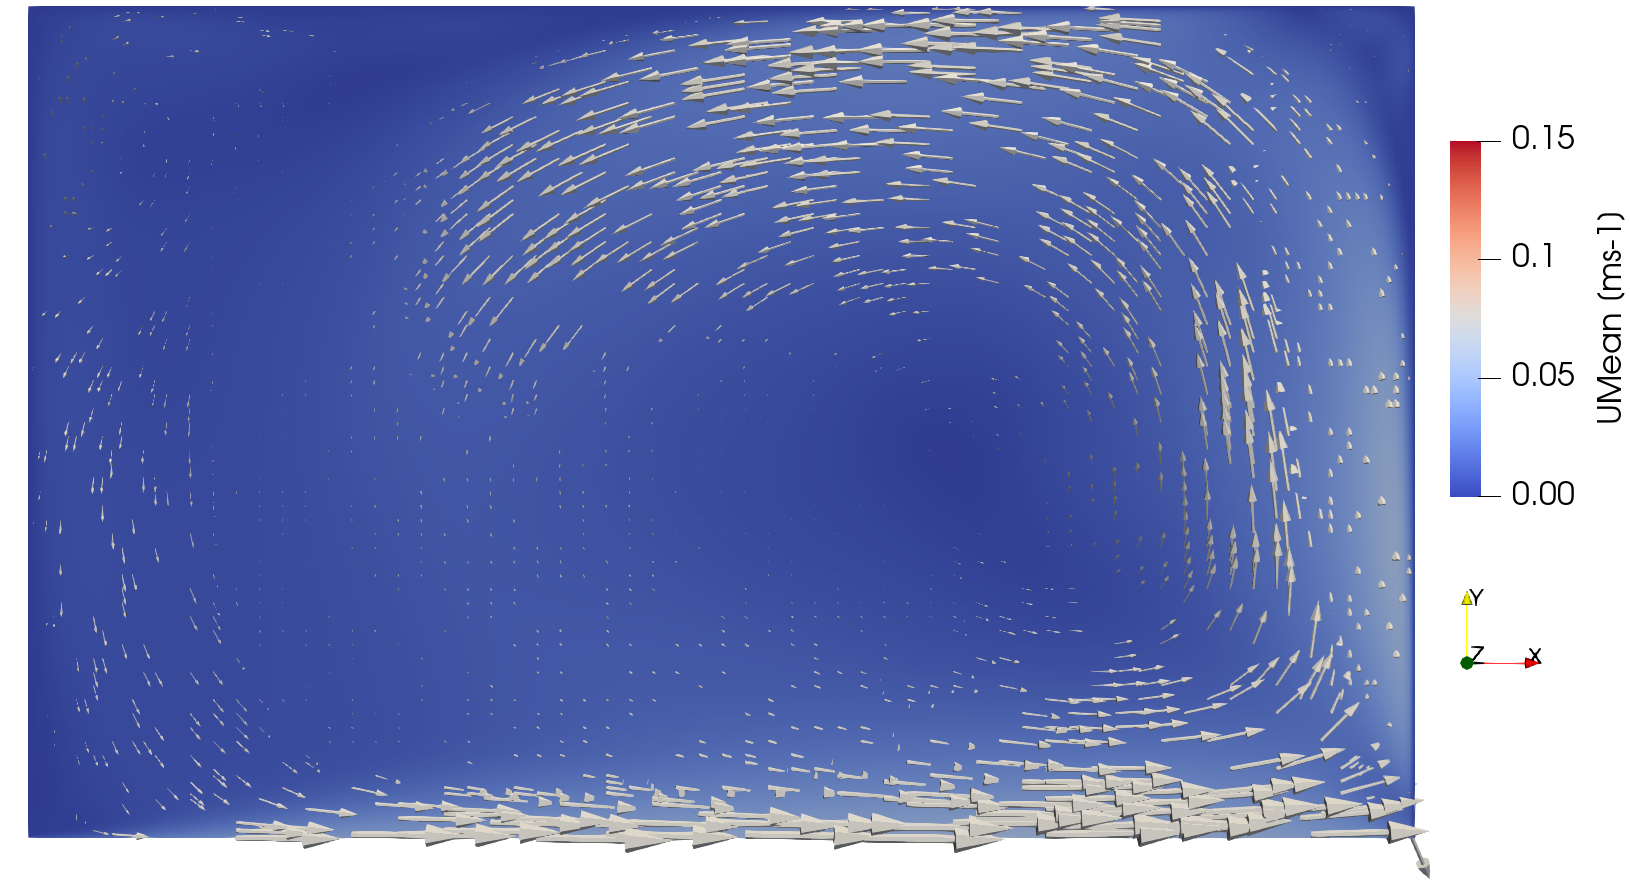
\includegraphics[width=\linewidth]{../images/art3/imgEst4.png}
\caption{Mean velocity vectors in the XY plane, in $z=0.6H$}
\label{fig:art3:vectors}
\end{figure}
The proposed model presented similar results when compared to numerical and experimental data. The ensemble average procedure was implemented to condense the values from the $0.6H$ plane to a single line capable to describe the internal behaviour of the cavity (\ref{fig:art3:graph}), where $y_0$ represents the beginning of the cavity. Notice that the model well predicts the flow except for the region close to $(y-y_0)/H=1.5$, this occurs due to the size of the computational cells in the region, a further refinement in this region could decrease the difference to experimental values. Although, it is important to highlight that the model obtained a high precision taking in account the much lower number of elements in the grid (\cite{xiang2019} model: $1.5\times 10^7$ elements; presented model: $1.4 \times 10^6$ elements), what represents a faster execution and a less intensive computational usage. The anti-clockwise circulation tendency is confirmed by the velocity profile in the farthest region from the main channel that presented negative velocities and the close to the interface ($0<(y-y_0)/H<0.6$), positive velocities. The circulation centre, region in which the velocity is zero were dislocated when compared to a lateral cavity without vegetation such as found in \textcite{gualtieri2010}, in which the centre occurs at the cavity centroid. Although,  in the vegetated case there was a displacement to the right, that accords to the higher velocity magnitudes inside the cavity. Albeit there was a displacement to the right in the x-axis, there was none in the y-axis, that can be verified with the contours from \ref{fig:art3:streamlines} and with position of the velocities close to zero ($0.6<(y-y_0)/H<0.82$).
\begin{figure}[!ht]
\centering
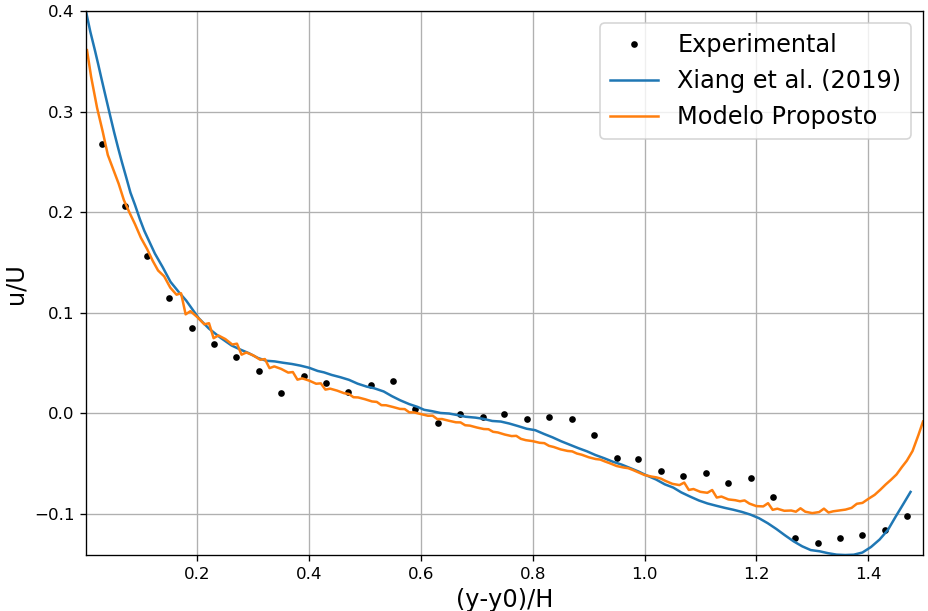
\includegraphics[width=\linewidth]{../images/art3/imgEst5.png}
\caption{Comparison of the ensembled averaged mean velocity $u$ in the XY plane, in $z=0.6H$}
\label{fig:art3:graph}
\end{figure}
\section{Conclusion}
The numerical model of a vegetated lateral cavity presented a good accuracy when compared to experimental data from literature. The method of anisotropic porous media can be considered an effective approach to reproduce the qualitative and quantitative aspects of the model at a lower computational cost when compared to conventional techniques. This validated mode, can represent a new way to study cavities and be the basis of more detailed investigations.
\section*{Funding}
This study was financed in part by the Coordenação de Aperfeiçoamento de Pessoal de Nível Superior - Brazil (CAPES) -Finance Code 001.
\addcontentsline{toc}{section}{References}
\printbibliography[segment=\therefsegment,heading=subbibliography, title={References}]
